% Michal Kovac's master thesis
%
\documentclass[a4paper,12pt]{book}
\usepackage{pgf}
\usepackage[utf8]{inputenc}
%\usepackage{a4wide}
% Now, switch on what is appropriate for czech:

% czech quotation marks
% \bq - begin quotation, \eq - end quotation
\def\bq{\mbox{\kern.1ex\protect\raisebox{-1.3ex}[0pt][0pt]{''}\kern-.1ex}}
\def\eq{\mbox{\kern-.1ex``\kern.1ex}}
%\setlanguage{\czech}

{%                                      % Begin a group for which " is active
\catcode`\"=\active                     % Make " an active character
\catcode`\@=11                          % Make @ an active character
%
%  \csdoublequoteson
%
%       This macro makes " an active character, resets the control sequence
%       \dblqu@te to L (left), and defines \dq as a replacement for ".
%
\gdef\csdoublequoteson{%                % \csdoublequoteson enables "
    \gdef"{\czechquotes}%               % Define " as \czechquotes
    \global\catcode`\"=\active%         % Make " an active character
    \global\chardef\dq=`\"%             % Double-quote char. via \dq
    \global\let\dblqu@te=L%             % Always start with a left double-quote
    }                                   % End of macro
%
%  \bq, \eq
%
%      These macros define default characters for czech left and right
%      double quotes. Czech opening quote is created from two commas with
%      kerning depending on fontdimen four parameter of current font.
%      Better solution should be specially designed character with
%      proper kernings; if you have such characters in fonts
%      (e.g. in DC-fonts), use it instead. (e.g. define
%      macros \bq and \eq e.g. \def\bq{\char"130 }
%      in your document/style file-- not in csquote.sty!)
%      Similar solution is used for czech right quote.
%
%      \cs existence test, stolen from TeXbook exercise 7.7
\def\ifundefined#1{\expandafter\ifx\csname#1\endcsname\relax }%
%
%      another macro to be more efficient in time and space
\global\chardef\f@@r=4
%
\ifundefined{bq}%
\gdef\bq{\kern-.25\fontdimen\f@@r\font,\kern-.8\fontdimen\f@@r\font,%
                \kern-.35\fontdimen\f@@r\font}%
\fi
\ifundefined{eq}%
\gdef\eq{\kern-.35\fontdimen\f@@r\font`\kern-.8\fontdimen\f@@r\font`%
                \kern-.25\fontdimen\f@@r\font}
\fi
%
% Macro \uv for other usage of \bq and \eq.
%
\ifundefined{uv}%
        \gdef\uv#1{\bq #1\eq}
\fi
%
% \testquotes macro gives warning if citation span this place
%
\gdef\testquotes{\if R\dblqu@te
        \message{Warning: You forgot right double quote!}%
        \let\dblqu@te=L\fi}
%
%  Define the macro that will be executed whenever " is encountered.
%
\gdef\czechquotes{\protect\czechqu@tes}
\gdef\czechqu@tes{%
        %  If the double-quote is the first character in a new paragraph,
        %  make sure it becomes a left double-quote.  This case can be
        %  detected by checking to see if TeX is currently in vertical mode.
        %  If so, the double-quote is at the beginning of the paragraph
        %  (since " hasn't actually generated any horizontal mode tokens
        %  yet, TeX is still in vertical mode).  If the mode is vertical,
        %  set \dblqu@te equal to L.
        %
        \ifinner\else\ifvmode\testquotes\fi\fi%
        %
        %  Now insert the appropriate left or right double-quote.
        %
        %  If \dblqu@te is L, insert an opening quote and set \dblqu@te to R.
        %
        \if L\dblqu@te\bq\global\let\dblqu@te=R%
        %
        %  Otherwise, save the current \spacefactor, insert '', set \dblqu@te
        %  to L, and reset the original \spacefactor.
        %
        \else%
           \let\xxx=\spacefactor%               % Save the \spacefactor
           \eq%                                 % Insert ending quote
           \global\let\dblqu@te=L%              % and reset \dblqu@te
           \spacefactor\xxx%                    % Reset the \spacefactor
        \fi%                                    % End of \if L\dblqu@te...
        }                                       % End of " macro
}                                               % End of group

\gdef\csdoublequotesoff{%
        \catcode`\"=12%                         % Set " back to other
        }
%
% Czech quotes are default
%
\csdoublequoteson




\pgfdeclareimage[interpolate=true,height=7cm]{faktorial}{faktorial}
\pgfdeclareimage[interpolate=true,height=7cm]{designimage}{designB}
\pgfdeclareimage[interpolate=true,height=3cm]{designimageSmall}{designB}
\pgfdeclareimage[interpolate=true,height=3.5cm]{creatorFactoryimage}{creatorFactory}

\author{Michal Kováč}
\title{User-oriented language for powerful data mining with Ferda}
\date{\today}

\begin{document}
\maketitle

\begin{description}
 \item [Název práce:] Uživatelsky orientovaný jazyk pro řešení úloh DZD
 \item [Autor:] Michal Kováč
 \item [Katedra (ústav):]
 \item [Vedoucí diplomové práce:] Doc. RNDr. Jan Rauch, CSc.
 \item [E-mail vedoucího:] Rauch@vse.cz
 \item [Abstrakt:]
 \item [Klíčová slova:]
\end{description}

\medskip

\begin{description}
 \item [Title:] User-oriented language for solving KDD tasks
 \item [Author:] Michal Kováč
 \item [Department:]
 \item [Supervisor:] Doc. RNDr. Jan Rauch, CSc.
 \item [Supervisor's e-mail address:] Rauch@vse.cz
 \item [Abstract:]
 \item [Keywords:]
\end{description}
\newpage

\tableofcontents

\section*{Zadání}
Východiskem diplomové práce jsou zkušenosti s GUHA procedurami implementovanými v rámci systému LISp-Miner [1]. Díky jak rozmanitosti vztahů které lze jejich pomocí hledat tak i vzhledem k rozsáhlým možnostem zadávání množiny potenciálně zajímavých vztahů lze pomocí těchto procedur hledat odpovědi na různé analytické otázky formulované způsobem blízkým přirozenému jazyku. Příkladem takové otázky je: \uv{Za jakých okolností a pro které pacienty není pravda, že s rostoucí úrovní cholesterolu roste i úroveň trigliceridů?}. Na tuto otázku lze hledat odpovědi pomocí procedur 4ft-Miner, SD4ft-Miner, KL-Miner i SDKL-Miner. Použitá procedura i způsob nastavení jejích parametrů dává různé možnosti co se týče podrobnosti odpovědi. Zevrubná odpověď na takovouto otázku vyžaduje několik vzájemně provázaných běhů několika procedur. Jednotlivé běhy procedur odpovídají dílčím otázkám indukovaným položenou otázkou.

Lze pokládat řadu podobných otázek které konstituují jistou typovou úlohu. Příkladem podobné otázky k otázce výše uvedené je otázka \uv{Za jakých okolností a pro které pacienty není pravda, že s rostoucí úrovní vzdělání roste i spotřeba vína?}. Pro řešení jedné typové úlohy existuje systém vzájemně provázaných dílčích otázek a ty lze chápat jako příkazy vhodného jazyka, kterým uživatel řídí postup při řešení typové úlohy.

Jedná se o diplomovou práci kategorie \uv{výzkumný problém}. Jejím cílem je stanovit několik typových úloh a pro ně definovat výše naznačený jazyk pro řešení. Jazyk bude založen na použití GUHA procedur implementovaných v rámci systému LISp-Miner, případně na nových vhodných analytických procedurách. Součástí diplomové práce bude i prototypová implementace příkazů tohoto jazyka v rámci systému FERDA [2].

\section*{Guides}
The main task of this paper is to assess a set of several problems in KDD and present a possible solution via a new user-oriented language for Ferda system. The reach of the present paper, however, surpasses the assignment in its implications. Instead of a new language specific only for some KDD problems, a new generic language with much wider extensibility and usability has been created as a part of this thesis. The reason for going beyond the task was the present author's determination to present a more complex solution to the problem given. 

Instead of presenting first KDD problems and later describing a new language specific for these problems a new generic language is described at the beginning. The generic language resulted indeed from some KDD problems but it is not visible on the result, which is why it is not needed to start with examples in this paper.

The creation of a new more generic language independent of KDD was established as the first task, followed by demonstration of KDD problems and their solution using the given generic language and special KDD functions in addition. The method used for creation of the new language relied on the principle of other functional languages, while maintaining the basic requirements of recursive countability and the widest possible application on the KDD problems.

There are references from solution of KDD problems to features in the new language which are used for their solution. Therefore it is possible to read problems with their solution first, but it is not recommended for understanding the new language.

The new implementation of GUHA procedures that has been created as a part of \cite[diploma thesis of Tomáš Kuchař]{thesisKuchar} is used instead of LISp-Miner procedures which have been proposed. The new implementation of GUHA procedures is more generic and better integrated into Ferda system. LISp-Miner procedures are deprecated in Ferda system.

\section*{Structure}
The thesis is divided into four chapters. The first chapter introduces Ferda system. First, it discusses the history of Ferda and its implementation. Subsequently, it presents its functional view. The chapter shows that Ferda was from beginning designed for user-oriented functional programming and it describes what was missing in the Ferda system from the point of programming and extensibility before this thesis.

The second chapter goes into more detail and describes new features, functions and tools which can help making Ferda better user-oriented programing tool. To start with, it focuses on source files, the basic programming instrument, and how they are organized and how a code can be reused. Then several new basic functions are introduced with description of their pilot implementation. Modern programing methods are discussed in the last part of this chapter. Neither this chapter nor the first chapter are specifically oriented on knowledge discovery or data mining.

The third chapter is the core of this thesis. It shows examples from KDD and shows how it can be solved in Ferda system by functionalities introduced in the first two chapters. It also proposes new functionalities specific for KDD.

The last chapter summarizes previous chapters. It lists features which have been implemented as part of this thesis and features which have been proposed only.

\chapter{Introduction to the Ferda}
\section{History}
!-- History of GUHA, LISp-Miner --!

Michal Kováč, Tomáš Kuchař, Alexander Kuzmin and Martin Ralbovský started to work on the Ferda Data Miner in the year 2003. The project was lead by doc. RNDr. Jan Rauch. The basic aim of this project was creation a of a user-friendly user interface for the LISp-Miner project. It has been achieved, but the Ferda was created with future extensions in mind and the main parts of the application are independent of data mining at all.

Ferda is a user-oriented application for working with special visual objects called boxes. It is represented by a small square with an image inside. Boxes have sockets and a user can connect other boxes to these sockets. Boxes have functions, sockets are places for parameters for these functions. The Ferda Data Miner is Ferda with boxes for data mining.

!-- TODO vložit obrázek krabičky --!

Firstly, the boxes for data mining were written for the LISp-Miner generators. It was hardly extensible. Later Tomáš Kuchař as a part of his diploma thesis \cite{thesisKuchar} wrote his own implementation of basic GUHA procedures for the Ferda Data Miner.

Since the completion of the project, numerous new boxes have been created for special applications like decision trees, ontology mapping or relational data mining.

\section{Ferda Data Miner}
\subsection{Programmers view of Ferda system}

Base parts of Ferda have been written in C\# 2.0. Ferda runs on both .NET Framework and Mono. Some parts of new boxes use also Java platform. Ferda uses middleware Internet Communications Engine for a communication between its parts. Every part can be written in another language and run on another computer. For easier development, many third party libraries and applications have been used -- mainly NAnt, NUnit, NDoc, Netron Graphic Library and DockDotNet library. 

Ferda is under second version of General Public License. It allows everybody to use it for free, redistribute it, change the code (providing the results are still under the General Public License).

The aim of Ferda project was to create application which is internationalized, well documented, modular, user-friendly and conforms Microsoft standards in user experience. It is still in progress, but the Ferda is near to completion.

Ferda is a client-server application. Client executable is the FerdaFrontEnd.exe and we call that part FrontEnd. There is no single server executable; instead there are more separate modules which all can act as separate applications. FrontEnd communicates with all of them. Some of these modules implement boxes so we call them box modules, other are helper modules like the GUHA mining engine.

\noindent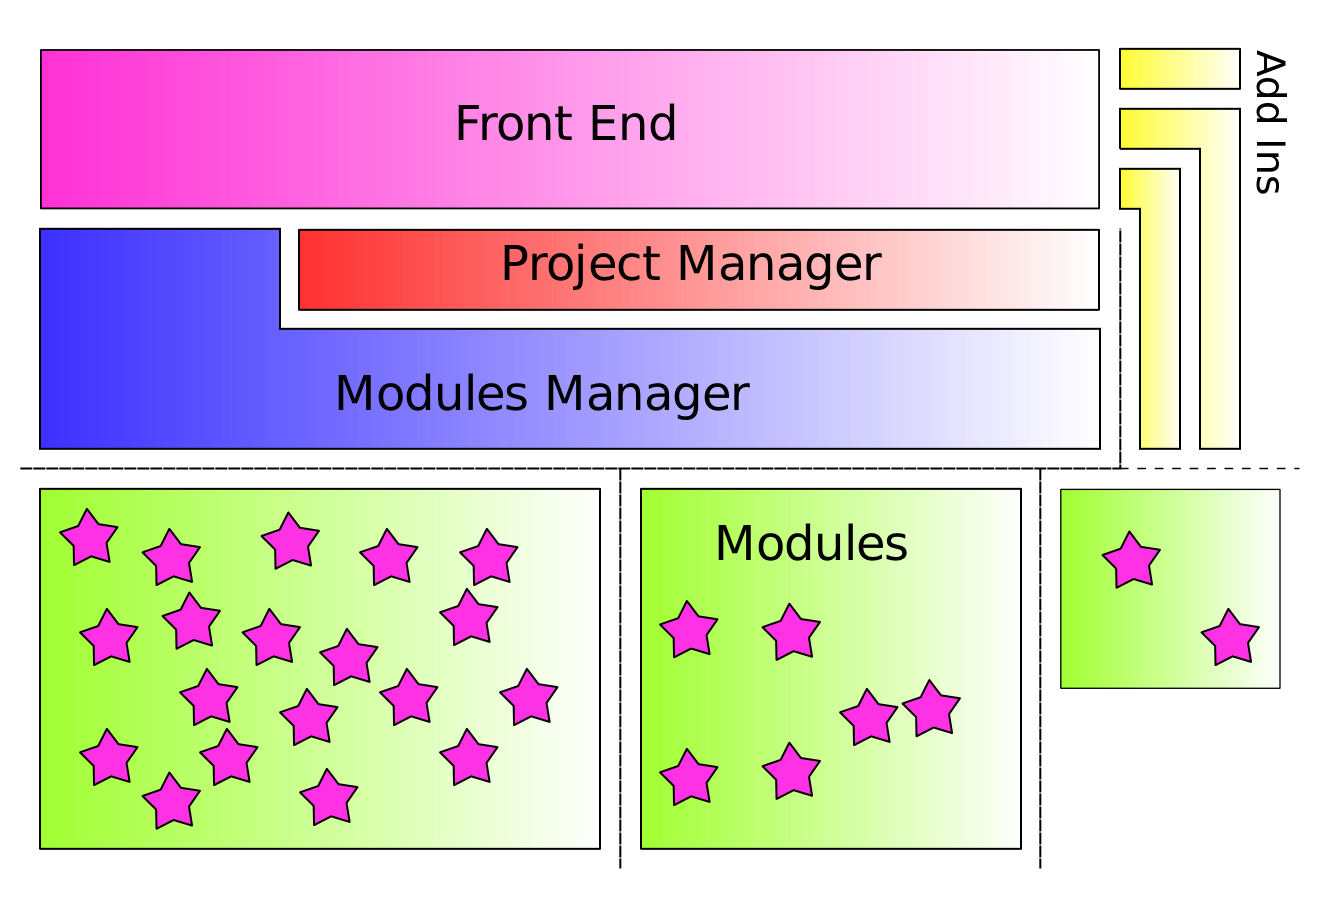
\includegraphics[width=13.72cm]{designB}

FrontEnd uses the assembly FerdaModulesManager.dll for a communication with modules. This assembly is layer of abstraction so that FrontEnd does not know that modules are not implemented locally (it hides Internet Communications Engine).

Another assembly that is used by FrontEnd is the FerdaProjectManager.dll. It controls projects. A project consists of an archive and views. The archive is a place for boxes. Views adds to boxes its placement on a desktop. Every box which is in the archive can be either in none or in one or more views. This manager is able to load a project from XML file and save it to XML file.

FrontEnd also loads add-ins. Add-ins can extend functionality of FrontEnd in many ways. Mainly it is used for modules for interaction and setting modules. Modules for interaction work on top of some box module. It for example shows results of functions returned by the box module. Setting modules are used for helping with setting nonstandard properties.

The communication between FrontEnd and modules and between modules itself is feasible via the Internet Communication Engine (ICE). ICE is a strong modern middleware. Thanks to the usage of ICE, Ferda is independent of both language and framework and it allows us to run different modules on different computers, but it does not add big complexity to the application. It can be also used for distributed computing.

IceGrid application, which manages available modules and loads them on demand, runs on a network. Modules manager uses these applications for getting modules.

Every box module implementation has its factory class. This factory class creates box module instances. There is one more layer -- every box module factory has its factory class, we call it box module factory creator, which is a singleton.

\noindent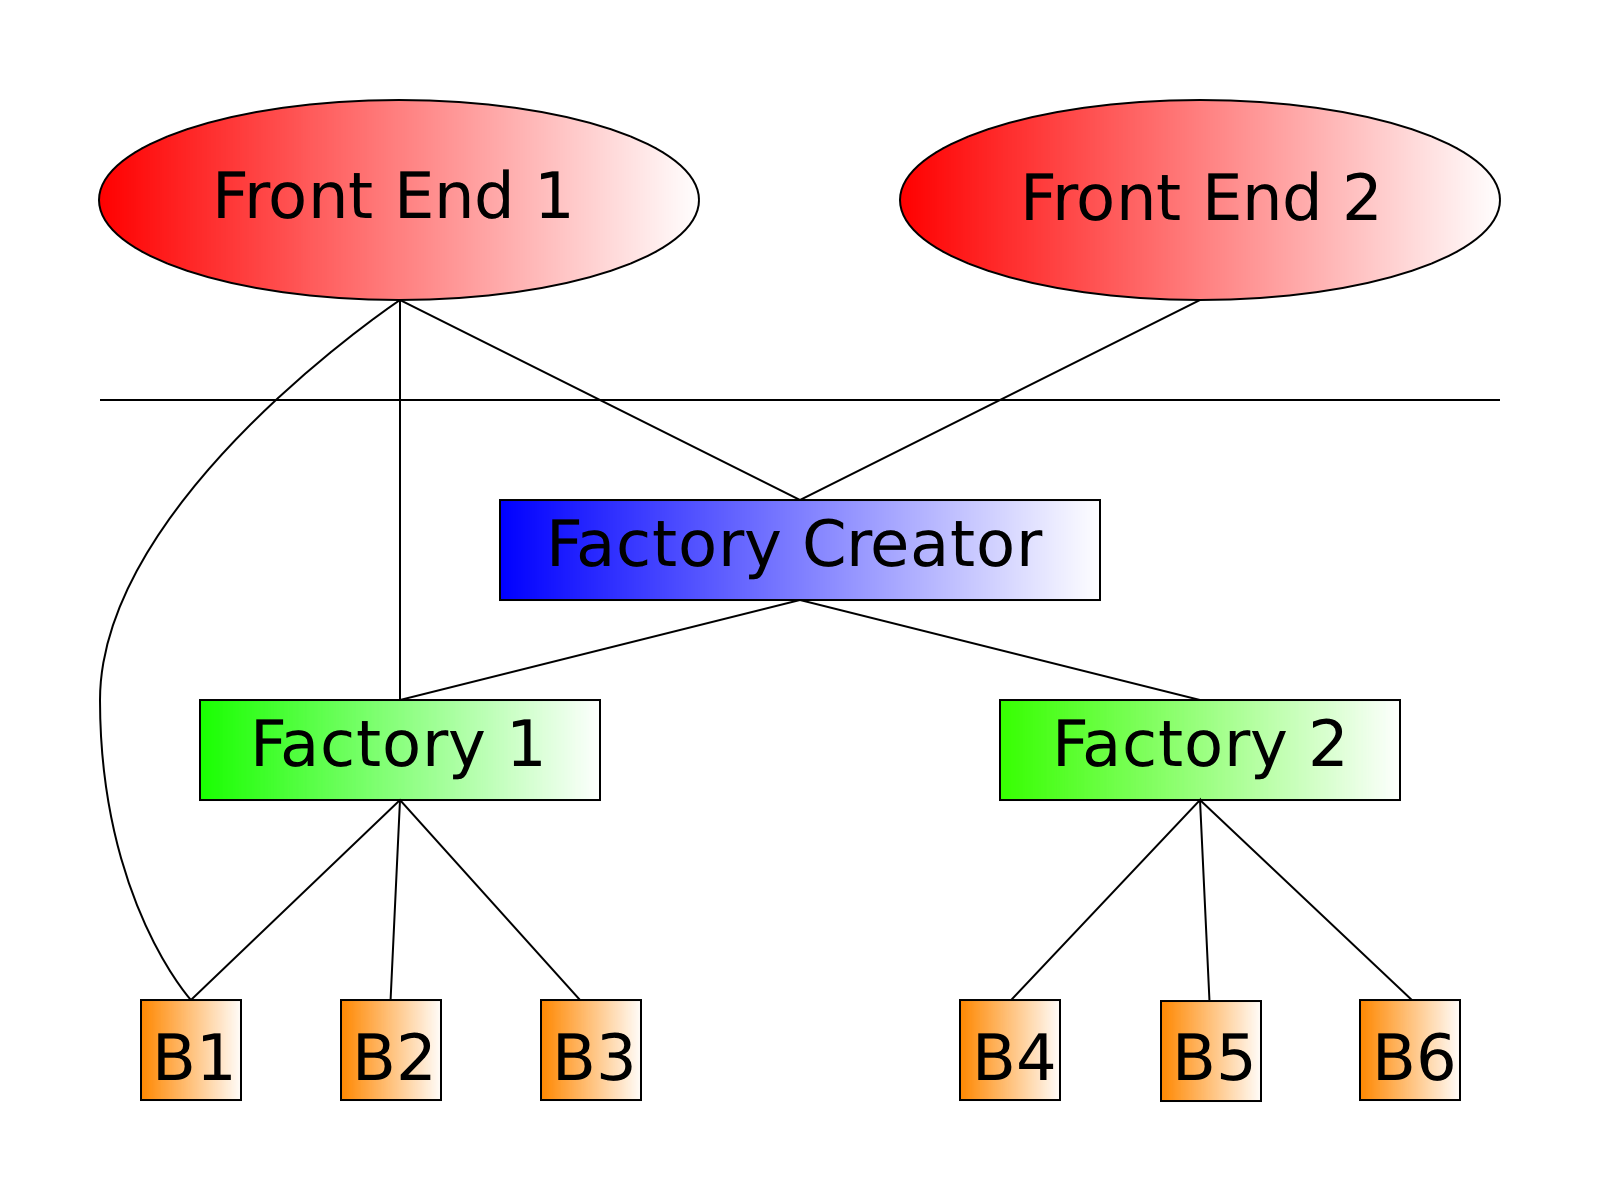
\includegraphics[width=13.72cm]{creatorFactory}

FrontEnd asks a box module factory creator for creation of only one box module factory for one box class. The creator has methods independent of both instance of the box module and FrontEnd connected. A factory has methods independent of box modules, but dependent on FrontEnd (for example localized names of properties). If FrontEnd is not connected for longer time, all factory instances and box module instances are destroyed.

Box modules mainly consist of sockets, properties and functions. Sockets are places where you can connect another box module. They are parameters for functionality of the box module. Properties are also parameters and can be viewed as a socket, but can be configured both by connecting a box to the socket and by setting the property in the property grid.

A box has a method which returns a class called functions. This class represents the functionality of a box.

Box module has also an identifier, an icon, a SVG design, names of categories, box modules asking for creation, actions, a name of property driving label and a dynamic help.

\subsection{Ferda as a programming language}
The main concept of Ferda is to be user-oriented functional language. The basic view is that a box is a function and sockets are properties of that function. There is no need to talk about properties, because properties are also usable by sockets. To be more precise, box can be not only viewed as one function, but as set of functions. As written above, box returns class functions. Therefore every method of such class can be viewed as a separate function. Box can also return different functions class depending on its parameters. We can define basic objects of the Ferda language.

Box is $\left<S,F\right>$ where
\begin{itemize}
	\item $S$ is a set of sockets
	\item $F$ is a set of functions
\end{itemize}
	
Socket is $\left<n,T\right>$ where
\begin{itemize}
	\item $n$ is socket name
	\item $T$ is a set of box types
\end{itemize}

We have predicate $has(f,i)$ where $f$ is function and $i$ is an ``Ice identifier''

Type is $\left<i,S\right>$ where
\begin{itemize}
	\item $i$ is an ``Ice identifier''
	\item $S$ is a set of $\left<n,i\right>$
	\begin{itemize}
		\item $n$ is socket name
		\item $i$ is an ``Ice identifier''
	\end{itemize}
\end{itemize}

Box $B=\left<S,F\right>$ is of type $A=\left<i,Z\right>$ iff 
\begin{enumerate}
	\item $(\forall \left<n,j\right>\in Z)(\exists \left<m,T\right>\in S)(\exists \left<y,W\right>\in T)(m=n \wedge j=y)$
	\item $(\exists f\in F)(has(f,i))$
\end{enumerate}
	
\begin{itemize}
	\item Box consists of functions
	\item Sockets are parameters of these functions
	\item Property is also socket
		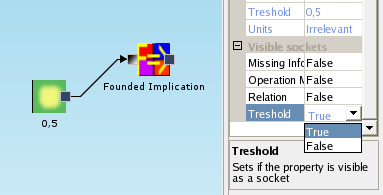
\includegraphics[width=7cm]{property_as_socket}
\end{itemize}

%What is missing?
%\begin{itemize}
%	\item Moving work from one project to another
%	\item Basic math boxes
%	\item Recursion
%	\item Other language boxes
%	\item Ferda specific language boxes
%	\item Data mining specific boxes for user programming
%\end{itemize}

\chapter{Language for visual programming}
\section{Source codes and reusability}
Every programming languages have ways how to reuse a code. 

\subsection{Project import}
The simplest way is to copy the source code to different place and use it for different project. The same is possible in Ferda, you can copy a project file and reuse it.

With standard textual source code it is easy to merge the code from more sources. You can do it with Ferda project, but you must merge a code in a project files manually in a text editor. The merging is not an easy process so it is not so much user-friendly way.

It would be nice have a functionality in Ferda that would allow us to import some or all boxes from one project into another one. One way to achieve that is adding a new item "import project\dots" to the Ferda menu. When a user selects this item, a dialog for selecting a project file should open. Having selected a project, the dialog with boxes in selected project should be shown. The user selects boxes which he wants to import. The last step is actual import of selected boxes.

Let us discuss the dialog box where a user selects boxes. It would be nice to see which boxes depend on which so that the user can chose whole functions. When he selects to import a box without a box connected to this box, the box will be imported, but the result of such box can be different than before. On other hand it can be on purpose, because user can want to connect to that box some box from original project.
% - zlepsit citelnost

% (or box connected to box connected to\dots connected to this box -- I will call this indirect connection) 

\subsection{Project using}
Source code of one application is mostly not written only in one source file, but in many. There are more ways in programming languages how to achieve this. One way typical for compiled languages is compilation of application from more source files from the beginning. A compiler as an argument has a set of files. Another way is that source code can import another source file. It is mostly used by interpreted languages. An advantage of this approach is that the imported file is loaded when it is used - so the file can be created a short time before usage. It allows us to write code which loads every file in some directory so that it can be used for plug-ins. Even compiled applications have a way how to achieve this functionality. Compiled applications can use libraries (or assemblies or modules) which can be loaded dynamically on demand. It can be also used for loading a source file on demand if a compiler for that language is available in machine where the application is being executed.

If we want to add this to Ferda, project has to have new attribute defining using of other projects. Boxes from these project should be read only -- no change of properties and boxes connected to theirs sockets is available. It should be visible from which project which box is used. If you remove a box from a project used by a box from another project which use the first project you should still somehow work with the second project without loosing the information about connection to non existing box. If you later add back the box to used project it should work again. It raises question how to add back the box. What should identify a box from used projects? At this time boxes are identified in one project by project identifier. The project identifier is integer which is growing from one up which user is not aware of.
%KONCIM S KLAROU

If user remove a box with last project identifier, exit Ferda, start Ferda, reopen the project and add a new box, the box can have the same project identifier as it had the removed box. If we want still to use project identifier as identification of boxes we should avoid this by serializing the last used project identifier in a project. Another functionality which can be wanted is ability to replace a box by another one. It means ability to delete box and create a new one which have the same project identifier.

%tady by mohlo byt jak by melo vypadat menu
\subsection{Defining function}
versus lambda expression - the same
\subsection{Name spaces}
\subsection{Network archive}
Another way how to reuse a box can be to copy it from another project. Let us have a new place where you can place boxes which you want to reuse. Such place can be on network and more users can place there theirs boxes and reuse them in another projects. They can use such place to move theirs work to others. Let us call this place network archive.

\subsubsection{Implementation}
As part of this thesis I have created a simple implementation of such network archive. The main part is a ICE service which is running somewhere on network. It has simple definition in slice:
\begin{verbatim}
interface Archive {
	/**
	 *
	 * Adds a box with connected subboxes to the archive
	 *
	 **/
	void addBox(Box boxValue, string label)
		throws NullParamError, NameExistsError;

	/**
	 *
	 * Removes the box from archive
	 *
	 **/
	void removeBox(string label)
		throws NameNotExistsError;

	/**
	 *
	 * Gets box which is in the archive
	 *
	 **/
	Box getBox(string label)
		throws NameNotExistsError;

	/**
	 *
	 * Gets labels of boxes in the archive
	 *
	 **/
	idempotent Ferda::Modules::StringSeq listLabels();
};
\end{verbatim}

Network archive is a collection of boxes (with all theirs sub-boxes -- boxes connected both directly and indirectly to that box). Each box is identified with some label. You can add a box and remove a box, get information about a box and list all labels in the collection. The collection is serialized on a disk every time it changes. After startup of the service it loads last serialized version.

From user perspective the network archive is a new panel with list where you can copy a box.
\begin{figure}
	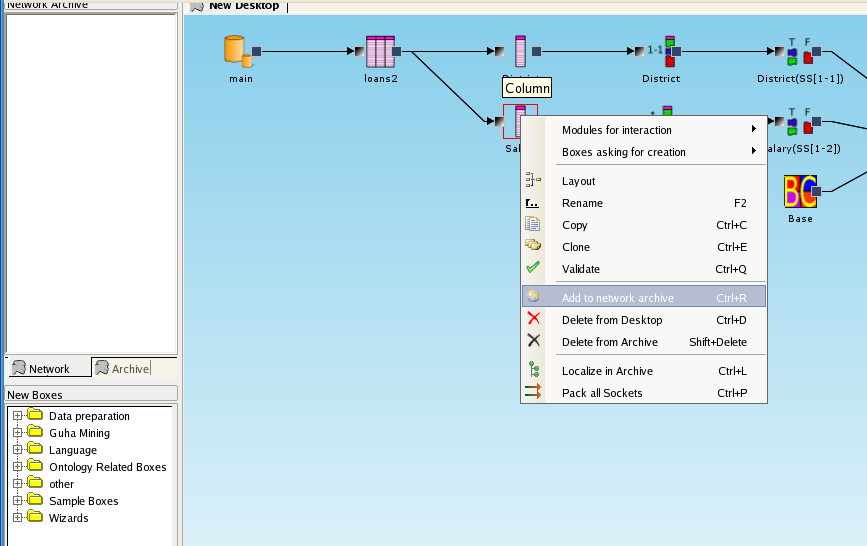
\includegraphics[width=13.72cm]{add_to_network_archive}
	\caption{Add a connection to the network archive}
\end{figure}
It will ask a user for entering a label after dragging a box from desktop to network archive.
\begin{figure}
	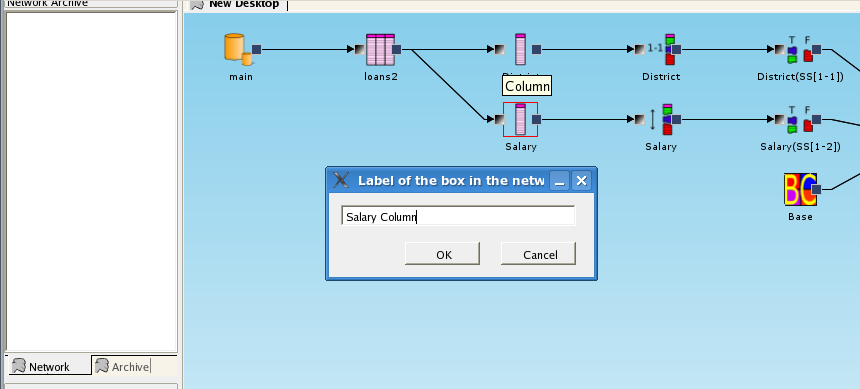
\includegraphics[width=13.72cm]{set_name_of_box_in_network_archive}
	\caption{Set a name of box in the network archive}
\end{figure}
After that in the list new item with selected label should be visible.
\begin{figure}
	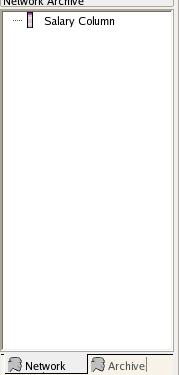
\includegraphics[height=7cm]{network_archive_box_added}
	\caption{New box added to the network archive}
\end{figure}
User can than go to another computer which use the same network archive and drag the box from network archive to another project. It should create a new copy of the box with all its sub-boxes on the desktop.
\begin{figure}
	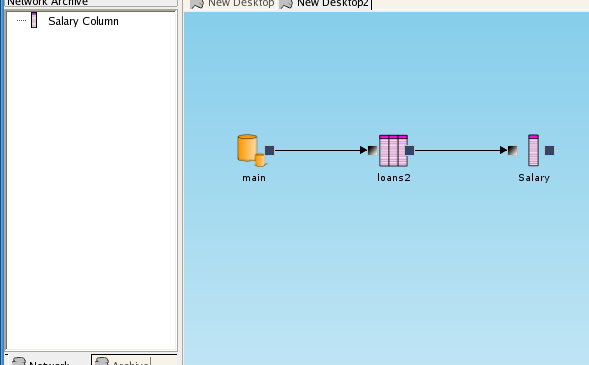
\includegraphics[width=13.72cm]{network_archive_drop_to_desktop}
	\caption{Drop box to a desktop from the network archive}
\end{figure}
He can also remove the box from the network archive.
\begin{figure}
	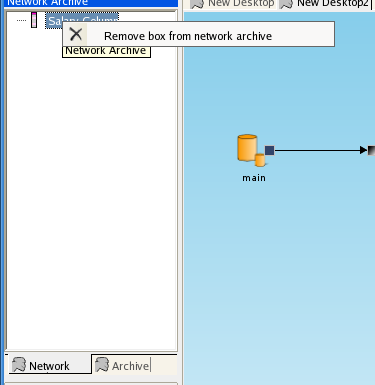
\includegraphics[height=7cm]{network_archive_remove_box}
	\caption{Remove box from the network archive}
\end{figure}

\subsubsection{Future enhancements}
It would be nice to organize boxes in network archives in some structure. It can be one level structure (labels) or tree structures like directories. Another enhancement would be to add user rights to these labels. Easy thing to do is to allow Ferda FrontEnd to work with more network archives.

\subsubsection{Summary}
Network archive is new place where a user can store connections. It is independent on projects. One network archive can be accessed from more computers. It is way how to move connections from one project to another.

\subsection{Summary}

\section{Functional languages}
%prvky - vzhledem k Ferdovi
%jak delaji rekurzi / lambdu - rozsil mezi structuralnim a funkcionalnim jazykem

\subsection{Lambda calculus}
Base of functional languages is in the lambda calculus. 

%rekurzivne spocetny
%vsecno je funkce
%typovany/netypovany

\section{Language boxes and expressions}
Every programming language has from beginning at least small set of functions. Also it has some way how to use these functions to create more complex ones. Such aparat has been created for Ferda as main part of this diploma thesis.

\subsection{Constants}
Ferda language is typed language. It means that functions in Ferda return values of some type. Easiest functions are constant functions which return specified value. There are at least two ways how to achieve this by box semantic. First way is to create for each type specific box for constants which returns that specific type. This type has been created in Ferda as a part of this thesis.

Second type is to create one box which have one property for specifying a type and dependent on it it has second property with value of specified type. It also returns that specified type.

\subsection{Boxes for math}
Mathematical expressions are really important for programmers, statistics and analytics. Support for them is important. New boxes for basic mathematic functions has been added. 

\subsubsection{Binary operation}
New boxes for basic binary operation has been added. It has first argument type of operation ($+$, $-$, $*$, $/$).
\begin{figure}
	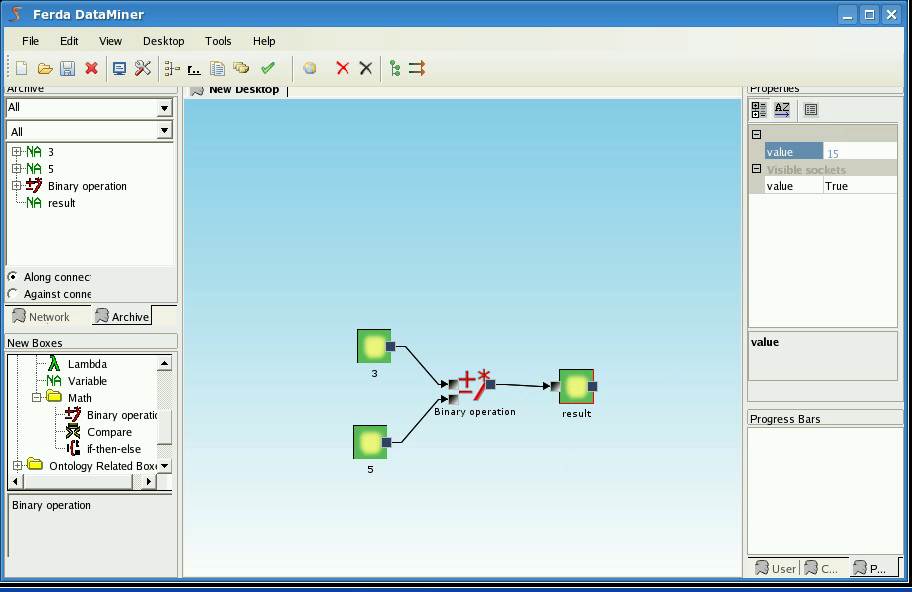
\includegraphics[width=13.72cm]{binaryOperation2.png}
	\caption{Binary operation}
\end{figure}

\subsubsection{Comparison}
Comparison functions are functions of two arguments which returns a boolean value. As part of this thesis compare box has been created which has three arguments. First argument is type of comparison function, next two arguments are doubles. This box has implemented basic mathematic comparisons ($<$, $>$, $<=$, $>=$, $=$, $!=$).
\begin{figure}
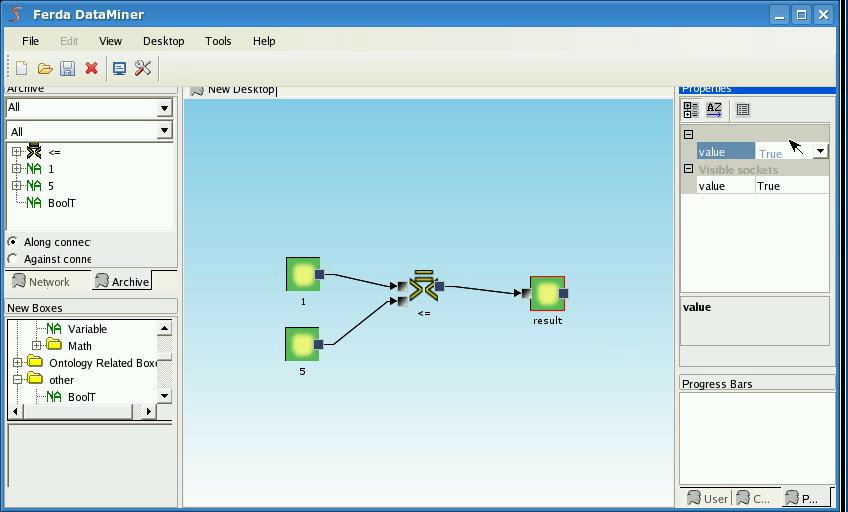
\includegraphics[width=13.72cm]{compare2.png}
	\caption{Compare}
\end{figure}

\subsubsection{If expressions}
If expression is a function which has three arguments. First argument is of boolean type. It returns value of the second argument if the first is true, otherwise it returns value of the third argument.
\begin{figure}
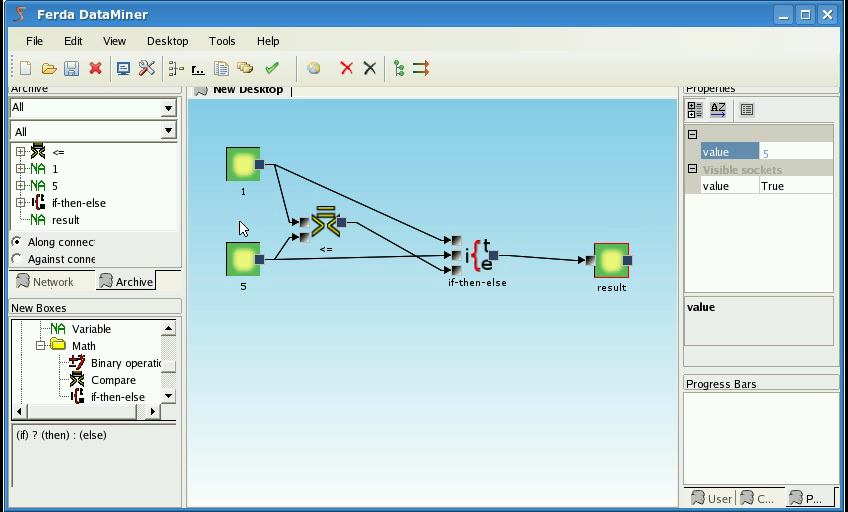
\includegraphics[width=13.72cm]{ifthenelse2.png}
	\caption{If expression}
\end{figure}

\subsection{Lambda expression}
Basic facts
\begin{itemize}
	\item From lambda calculus $(\lambda x.(1+x))(9)$
	\item Basics of functional programming
\end{itemize}

Lambda in C\# 3
\begin{verbatim}
public delegate int function(int x);

public static void Main(string[] args)
{
  function plusOne = x => 1 + x;
  var a = plusOne(9);
  System.Console.WriteLine(a);
}
\end{verbatim}
	
Other languages

Lambda in F\#
\begin{verbatim}
let onePlus x = 1 + x
do printf "%s" (onePlus(9)) 
\end{verbatim}

Lambda in Python
\begin{verbatim}
plusOne = lambda x: 1 + x
print plusOne(9)
\end{verbatim}

without parameters
\begin{figure}
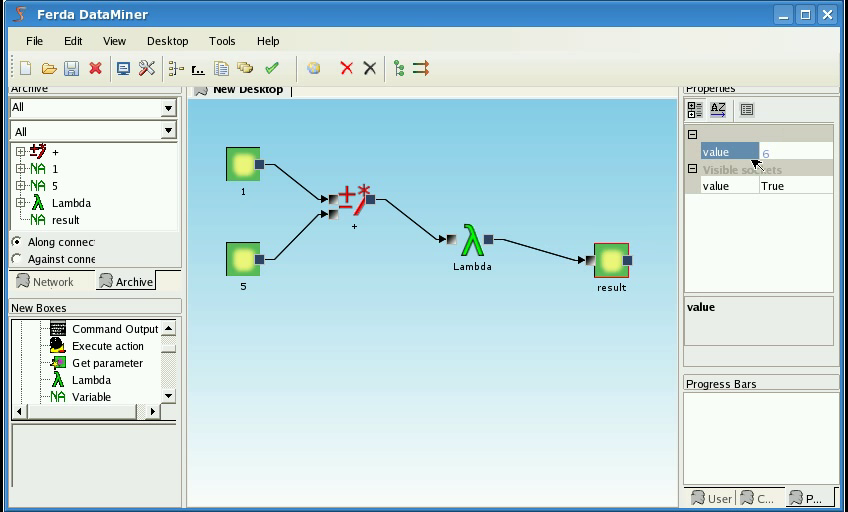
\includegraphics[width=13.72cm]{lambdaBasic2.png}
	\caption{Lambda without arguments}
\end{figure}

One constant parameter specified
\begin{figure}
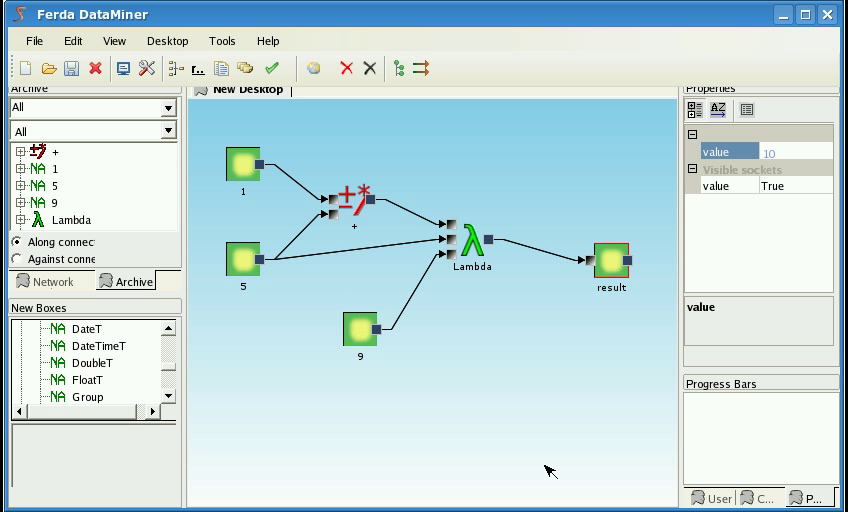
\includegraphics[width=13.72cm]{lambdaBasic3.png}
	\caption{Lambda with one constant parameter specified}
\end{figure}
	
\subsubsection{Implementation of lambda}
How it really works -- Algorithm
\begin{itemize}
	\item Values of variables are cloned (whole subtree)
	\item Main function is cloned with substitution and returned
\end{itemize}

\subsubsection{Example usage of lambda -- factorial}
Factorial in C\# -- Structural version

\begin{verbatim}
public static int Factorial(int x)
{
  if (x == 0)
  {
    return 1;
  }
  else
  {
    return x * Factorial(x - 1);
  }
}
\end{verbatim}
	
Factorial in C\# -- Expression version

\begin{verbatim}
public static int Factorial2(int x)
{
  return (x == 0) ? 1 : x * Factorial2(x - 1);
}
\end{verbatim}

Factorial in other languages

Python
\begin{verbatim}
fac = lambda x: x == 0 and 1 or x * fac(x - 1)
\end{verbatim}

F\#
\begin{verbatim}
let rec factorial n =
    if n=0 then 1 else n * factorial(n - 1)
\end{verbatim}
	
Factorial in Ferda
\begin{figure}
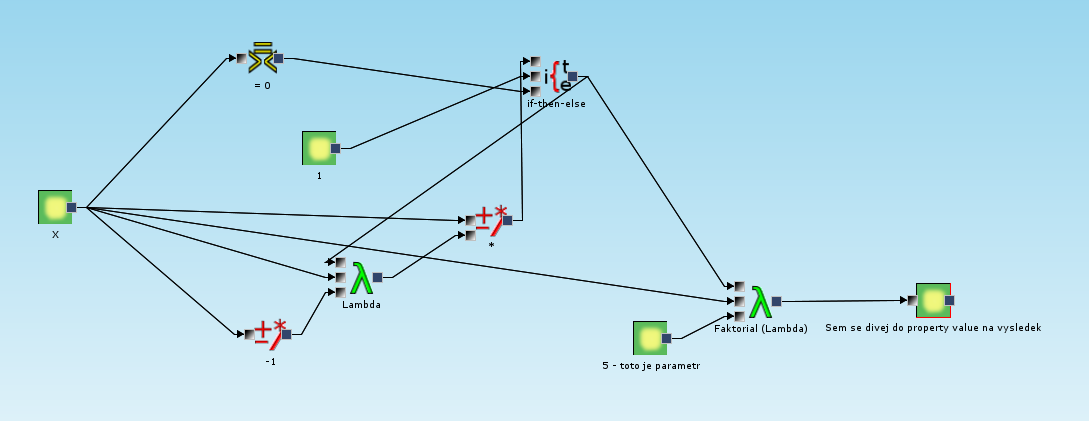
\includegraphics[width=13.72cm]{faktorial}
	\caption{Factorial}
\end{figure}
\subsection{Sequences and sets}
\subsection{Other new boxes}
\subsubsection{Get parameter}
\begin{figure}
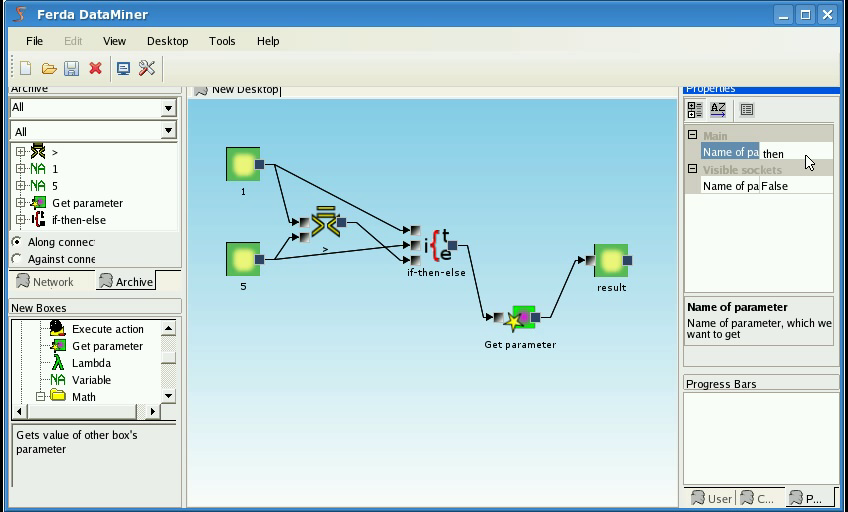
\includegraphics[width=13.72cm]{getParameter2.png}
	\caption{Get parameter}
\end{figure}

\subsubsection{Execute action}
\begin{figure}
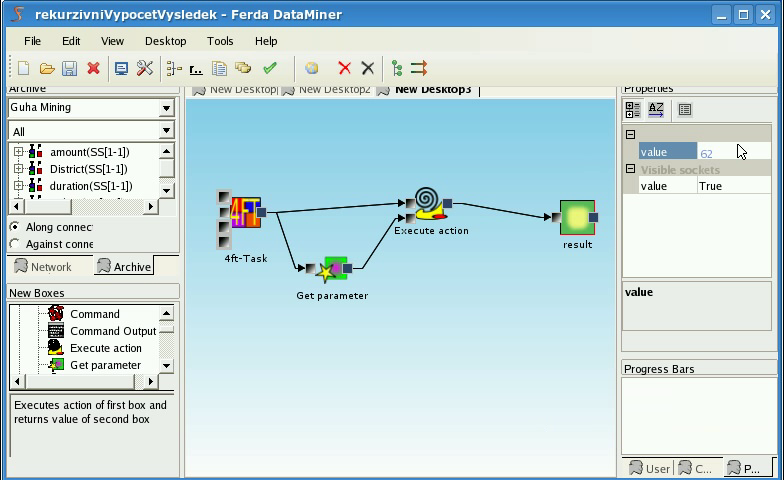
\includegraphics[width=13.72cm]{executeAction2.png}
	\caption{Execute action}
\end{figure}

\subsubsection{Command and command output}
\begin{figure}
	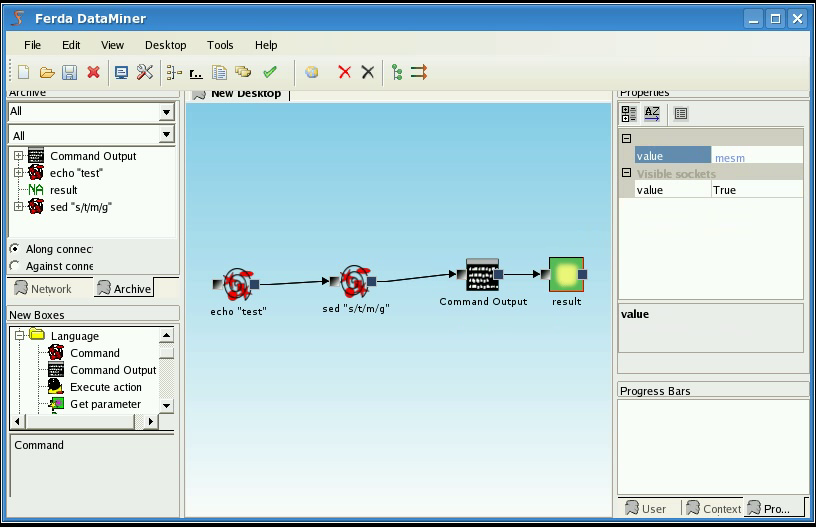
\includegraphics[width=13.72cm]{command2.png}
	\caption{Command and command output}
\end{figure}

The same in console
\begin{figure}
	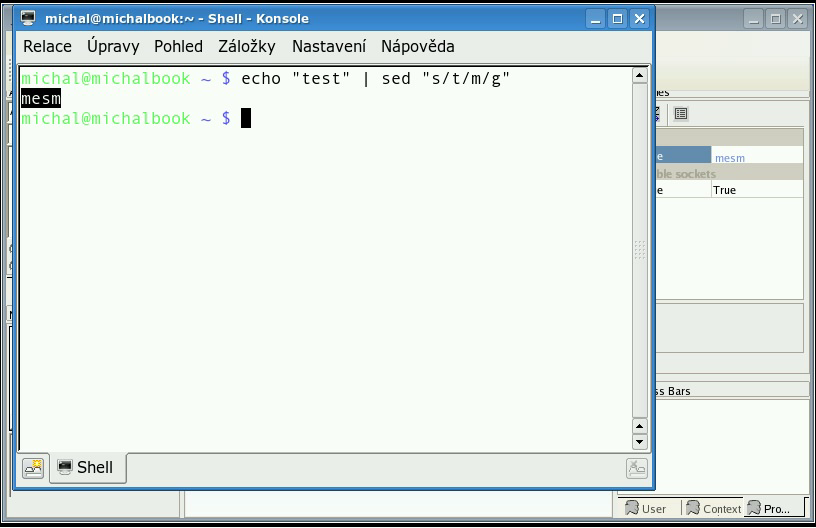
\includegraphics[width=13.72cm]{command3.png}
	\caption{Konsole version previous example}
\end{figure}
\section{Advanced tools and topics}
\subsection{Unit tests}
It would be nice to have a box called unit test, which should have a name and one socket for connecting assert boxes. Assert box should be a box which validates some condition and when the condition is not satisfied it should return some message describing the problem. Then there should be small application which takes a project as parameter and calls all unit tests in the project. Unit tests should call all asserts which are connected to the test. When any of them fail the application should return the message with name of unit test and the error message from the failed assert. Even though one unit test failed it should call other tests.

Similar is the NUnit tool for .NET Framework. For reusing tools which executes NUnit tests it would be nice to create generator of NUnit tests from Ferda project unit tests. Such generator should create one assembly for one project, but also so many test methods so many unit test boxes are in the project. There should be one startup method for initializing the Ferda Project Manager and for loading the project. 

\subsection{Exceptions}
%vyjimky a Ferda - uzivatel muze chytat a vysilat vyjimky
\subsection{Dependency injection}
Dependency injection is modern pattern in object oriented programming. You create a services and specify which services depends on which interfaces and later you set if needed which instances should be used. It is very useful for unit testing. In Ferda we can see a box with all it's sub-boxes as a service. Not set sockets are interfaces on which it depends (because of lambda box it is not needed to define it on sub-boxes).

\subsection{Aspect oriented programming}
\subsection{Distributed computation}
%vyber na kterem pocitaci ktera krabicka bezi
\chapter{KDD problems and theirs solutions}
\section{Four fold task in recursion}
\section{Getting basic information from table}
\section{GUHA in the Ferda by ``small'' boxes}
%Implementation of GUHA in Ferda by 'small' boxes.
%souvisi result browser - aby umel heterogenni vysledky - vystup z 4FT + vystup z CF

\section{\dots}
\chapter{Summary}
!-- co bylo uděláno, co bylo naprogramováno součástí této práce, strčný seznam návrhů do budoucnosti --!
%\section{Future tasks to do in Ferda}
%popis jednotlivych tasku s narocnosti, uzitkem - bodove ohodnotit

% modules for interacion je treba vylepsit


\begin{thebibliography}{thesisKuchar}
\bibitem{thesisKuchar} Tomáš Kuchař -- jeho diplomová práce
\bibitem{GUHA} GUHA book
\bibitem{ICE} Internet Communications Engine documentation
\bibitem{dalsi} \dots
\end{thebibliography}
\end{document}
